\section{Fully Connected Layer}
\label{sec:fc_layer}

In a Fully Connected Layer each perceptron is connected to each of the outputs of the previous layer.
Both the inputs and the outputs are organized as a one dimensional array.

The output of each perceptron is computed as an activation function of the weighted sum of all the inputs plus a bias.
The activation function aims to break the linearity of perceptron, allowing the successive layers to build increasingly complex non-linear features of the original input.
Common choices for the activation are the Sigmoid and the \ac{ReLU} function.

The Sigmoid function as the form:
\begin{equation*}
    f(x) = \frac{1}{1 + e^{-x}}
\end{equation*}
and can be seen in \cref{fig:sigmoid}.
It has the nice property that it is almost linear and quite steep in an interval of zero, which makes the learning process very quick.
On the other side, is saturates very quickly as soon as the input moves away from zero.
This can accidentally ``kill'' the perceptron, since the backpropagation algorithm multiplies the error from the following layer to the local gradient to calculate the weights update \cite{CS231n}.

\begin{figure}[ht]
	\centering
	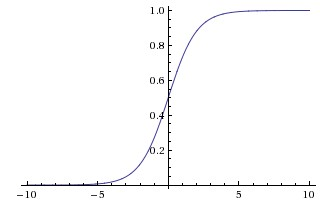
\includegraphics[scale=0.6]{figures/sigmoid}
	\caption{The Sigmoid function.}
	\label{fig:sigmoid}
\end{figure}

A popular alternative is the \ac{ReLU} function.
\ac{ReLU} is defined as follows:

\begin{equation*}
    f(x) = max(0, x)
\end{equation*}

and can be saw in \cref{fig:relu}.

\begin{figure}[ht]
	\centering
	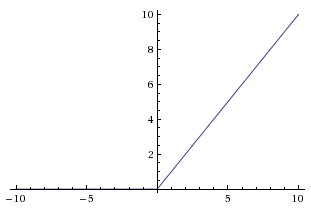
\includegraphics[scale=0.6]{figures/relu}
	\caption{The \ac{ReLU} function.}
	\label{fig:relu}
\end{figure}

\ac{ReLU} has been shown to greatly accelerate the learning process compared to the Sigmoid function \cite{krizhevsky2012imagenet}.
Another advantage is that it does not require to compute complex functions like exponentiation, but simply a threshold.
Unfortunately, \ac{ReLU} units suffer of the same ``dying'' problem of Sigmoid ones.
With high learning rates, the weights of the perceptron can be updated in such a way that its gradient become zero (and will never be updated again).
To reduce this problem, a proper choice the learning rate is necessary \cite{CS231n}.
